\documentclass[10pt,twoside,twocolumn,openany,bg=print,justified]{dndbook}

\usepackage[french]{babel}
\usepackage[T1]{fontenc}
\usepackage[utf8]{inputenc}
\usepackage{listings}
\usepackage{hyperref}
\usepackage{pdfpages}
\usepackage{parskip}
\usepackage{xkeyval}
\usepackage[export]{adjustbox}

\lstset{%
  basicstyle=\ttfamily,
  language=[LaTeX]{TeX},
}

\setlength{\parindent}{0pt}
\setlength{\parskip}{10pt}

\usepackage{xcolor}
\hypersetup{
    colorlinks,
    linkcolor={red!50!black},
    citecolor={blue!50!black},
    urlcolor={blue!80!black}
}



\begin{document}
\tableofcontents

\chapter{Don't Leave the Road, c'est quoi ?}

Il y a fort longtemps, un cataclysme a frappé le monde tel que nous le connaissons. Depuis, les humains tentent de survivre sur une Terre devenue hostile. Ils se sont terrés dans de petites communautés, reliés par des routes dangereuses qui balafrent des terres qui le sont encore plus.

Vous y incarnez des voyageurs. Des personnes qui, de plein gré ou non, se sont retrouvées sur les routes, et affrontent ou fuient les horreurs qui rôdent en dehors des communautés. Qui sait, peut être percerez-vous les secrets du monde d'avant.

Trois univers sont actuellement prévus pour Don't Leave The Road :

\begin{itemize}

  \item \textbf{Unterwald :} Depuis le cataclysme, la nature a repris ses droits sur les terres autrefois dominées par l'homme. Les créatures du règne animal ont muté dangereusement, et sont devenues particulièrement agressives, à l'exception notable de quelques-unes domestiquées par l'homme. Découvrez les secrets qui se cachent dans les vallées reculées. Il s'agit de l'univers présenté dans ce kit de découverte.
  \item \textbf{Les Voyageurs du Dehors :} Le cataclysme a déréglé quelque chose dans le climat. Fortement déréglé. Depuis maintenant plusieurs siècles, le monde est sous l'effet d'une puissante glaciation et les hommes se terrent dans des villes sous la glace, ou dans des cavernes. Une caste de puissants savants, les Arcanistes, gouverne les différentes communautés et protège ses secrets avec opiniâtreté.
  \item \textbf{Broken Stars :} Une immense station spatiale, qui dérive dans l'espace depuis des siècles, et qui semble s'agrandir à chaque nouvelle collision. Les habitants de cette station affirment que celle-ci est dotée d'un esprit propre, et que telle un prédateur, elle joue avec ses habitants. 

\end{itemize}

Don't Leave the Road est épaulé par un système simple, et des règles rapides à lire, afin de passer plus rapidement au jeu. Les règles ainsi que les univers cités ci-dessus sont sous licence libre Creative Commons, sont disponibles gratuitement.

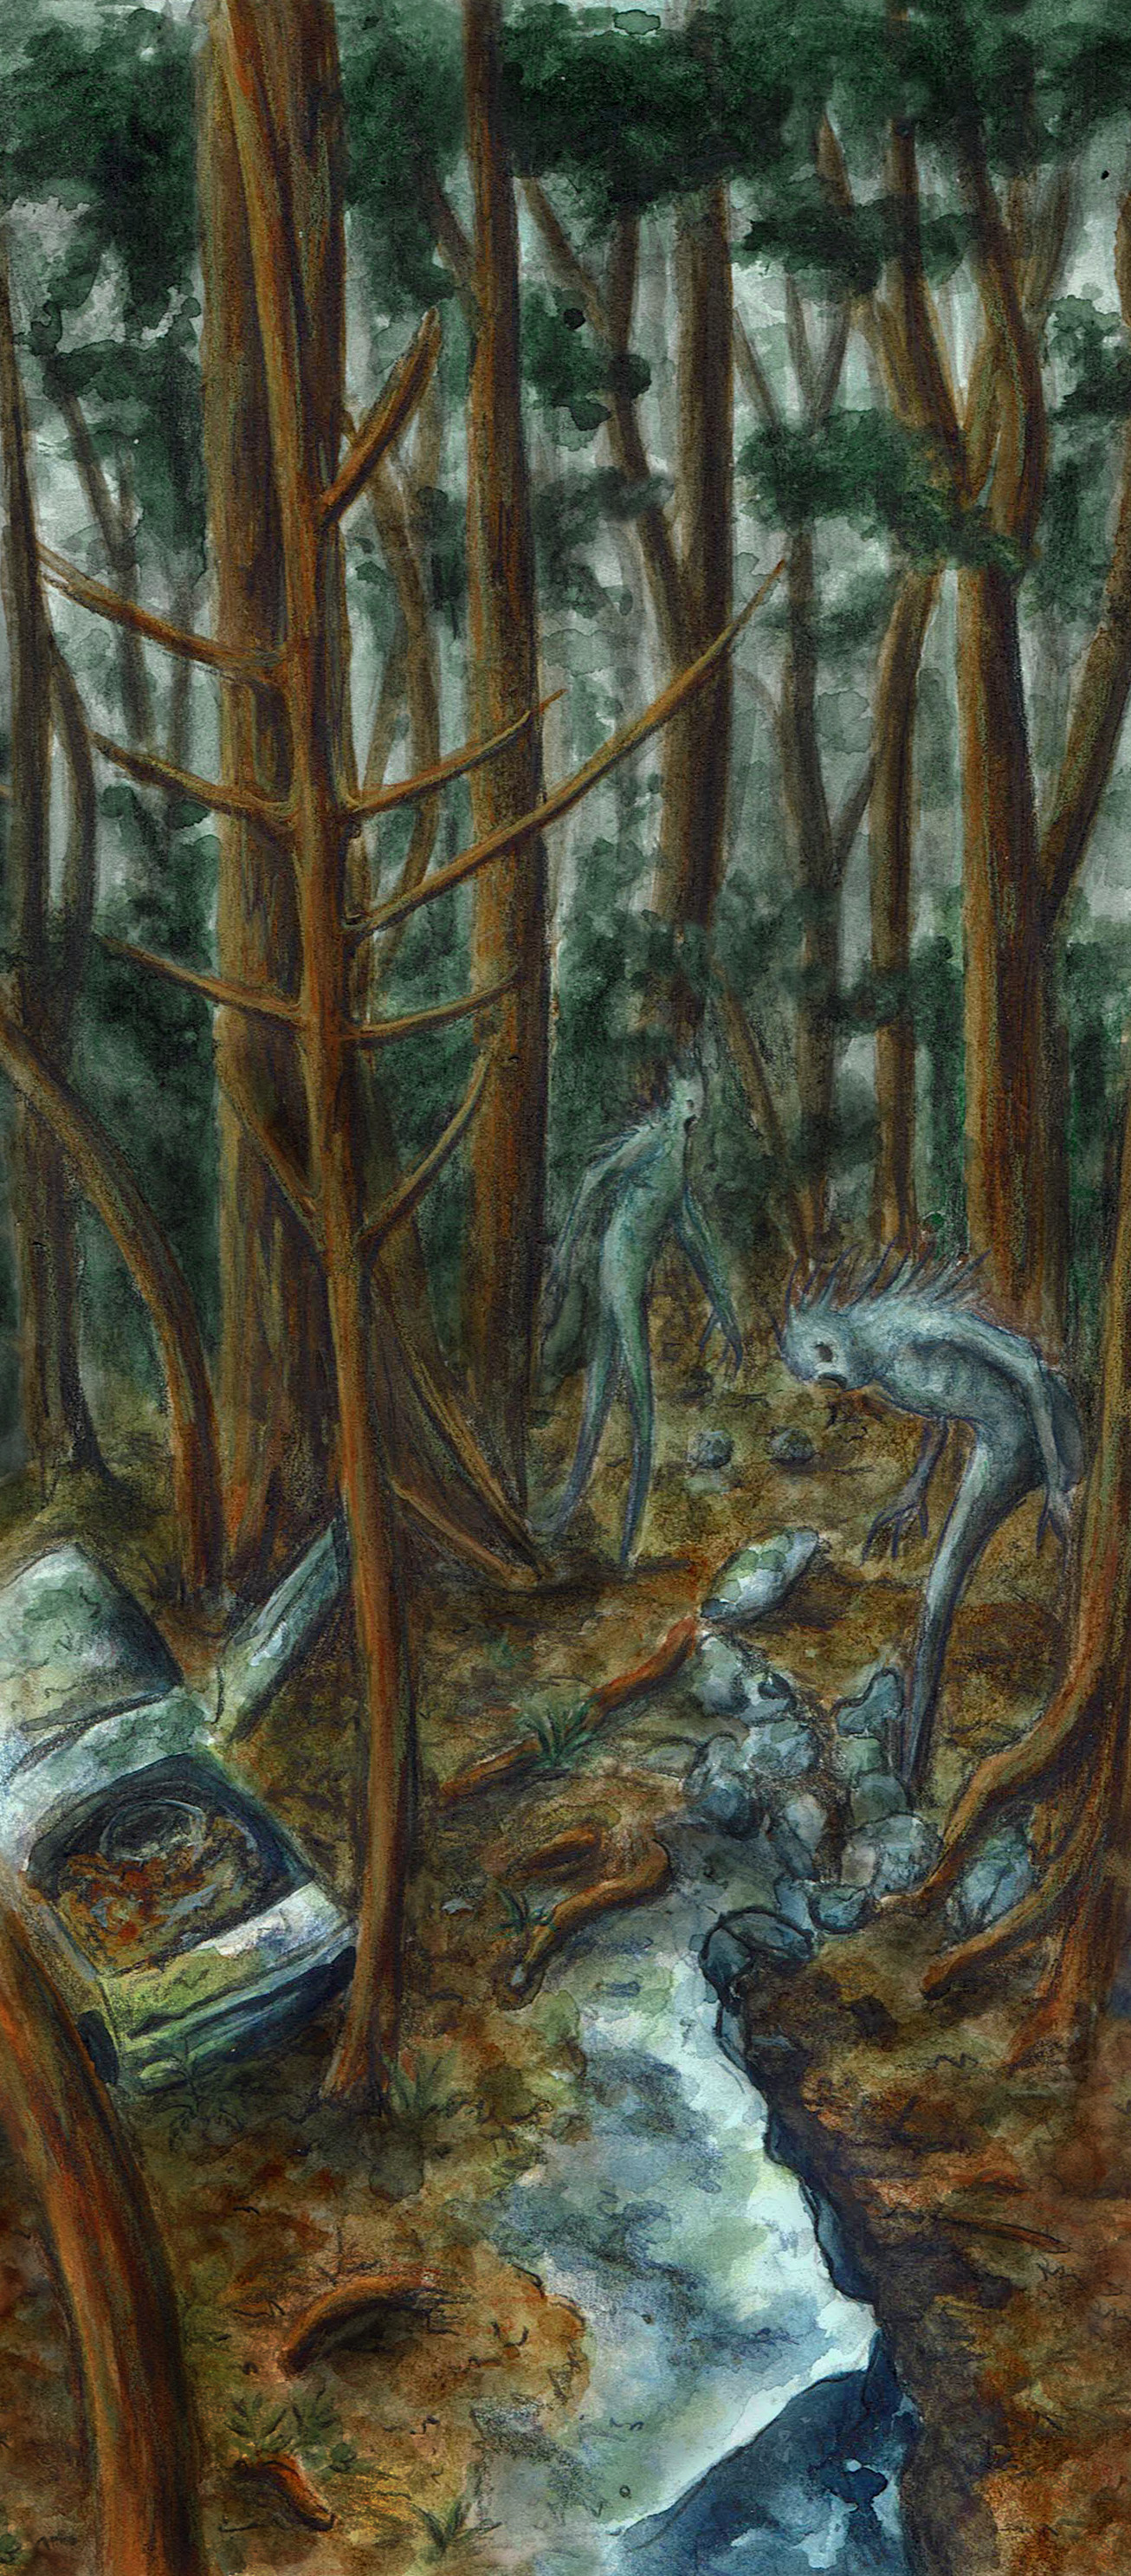
\includegraphics[width=\columnwidth, keepaspectratio]{img/monstre_foret.jpg}

\chapter{Comment jouer ?}

Le système de jeu se veut très simple et axé sur la narration plus que sur des jets de dés à répétition. Le d12 est le principal (seul) dé utilisé. 

\section{Caractéristiques}

Les caractéristiques sont au nombre de 3 :

\begin{itemize}
	\item \textbf{Corps :} Pour toutes les actions physiques et la résistance aux chocs.
	\item \textbf{Esprit :} Pour les actions mentales et la résistance à la folie et à la peur.
	\item \textbf{Âme :} Pour les actions sociales et la résistance aux intimidations et mensonges divers et variés.
\end{itemize}

La valeur d'une caractéristique se situe entre 0 (amorphe ou mort) et 12 (surhumanité totale). La moyenne humaine d'une caractéristique est de 5.

\newpage

\subsection*{Le Corps}

La caractéristique de Corps représente son aptitude physique. Un personnage fort, agile ou résistant sera donc doté d'un Corps élevé. Par opposition, une personne à la santé fragile ou maladroite aura un Corps faible. La réserve de Corps est également la santé physique, qui diminue lorsque le personnage se fait blesser physiquement.

\begin{dndtable}
\textbf{Valeur de Corps} & \textbf{Description} \\
12 & Surhumain. Il n'est pas difficile de défoncer des murs de forteresse ou de courir sur l'eau. \\  
10 & Extrêmement fort. Vous êtes invaincu au bras de fer depuis des années et les microbes fuient en vous voyant.\\ 
8 & Très fort, agile et endurant. Maximum à la création. \\
5 & Moyenne humaine \\
3 & Faiblard. Minimum à la création
\end{dndtable}


\subsection*{L'Esprit}

La caractéristique d'Esprit représente son aptitude mentale. Un personnage intelligent, astucieux ou attentif sera donc doté d'un Esprit élevé. Par opposition, une personne à la intelligence limitée ou peu réceptif aura un Esprit faible. La réserve d'Esprit est également la santé mentale, qui diminue lorsque le personnage est confronté à des événements traumatisants, ou se fait attaquer psychiquement.

\begin{dndtable}
\textbf{Valeur d'Esprit} & \textbf{Description} \\
12 & Surhumain. Votre esprit surentraîné détecte les moindres incohérences, et votre perception est meilleure que celle du plus terrible prédateur. \\  
10 & Extrêmement doué. Vous pouvez résoudre des problèmes logiques en un instant et vous avez un oeil d'aigle.\\ 
8 & Très intelligent et perceptif. Maximum à la création. \\
5 & Moyenne humaine \\
3 & Myope comme une taupe ou stupide. Minimum à la création
\end{dndtable}

\subsection*{L'Âme}

La caractéristique d'Âme représente son aptitude sociale. Un personnage charismatique ou beau sera donc doté d'une Âme élevée. Par opposition, une personne laids ou effacée aura une Âme faible. La réserve d'Âme est également la santé sociale, qui diminue lorsque le personnage se fait blesser socialement, comme lors d'un duel d'éloquence.

\begin{dndtable}
\textbf{Valeur d'Âme} & \textbf{Description} \\
12 & Surhumain. Votre verve et votre beauté sont révérées dans les légendes. \\  
10 & Extrêmement charismatique. Il suffit que vous entriez dans une auberge pour que tous les regards se tournent vers vous.\\ 
8 & Très beau, charismatique et avec une belle verve. Maximum à la création. \\
5 & Moyenne humaine \\
3 & Laid ou effacé. Minimum à la création
\end{dndtable}

\subsection*{Valeur et réserve de caractéristiques}

La valeur de caractéristique est (pour un nouveau personnage) le nombre de points attribués à la caractéristique.

La réserve de caractéristique est le nombre actuel de points qu'a le personnage dans sa caractéristique. Elle monte et descend lors de l'histoire.

Lorsque la réserve de caractéristique arrive à 0, le personnage n'est plus jouable. Le joueur doit alors créer un nouveau personnage. À 0 de Corps, un personnage est mort, rekt, fini quoi. À 0 d'Esprit, il est complètement fou. À 0 d'Âme, il est catatonique et ne s'exprime plus que par grognements.

\subsection*{Prendre des dommages dans une caractéristique}

Lorsqu'un personnage subit des dégâts physiques, ceux-ci sont directement impactés dans sa caractéristique de Corps.

Lorsqu'il subit une grande peur ou des émotions mentales divergentes (par exemple, en étant attiré et révulsé à la fois par la bête qu'il voit), cela crée des dégâts mentaux qui sont impactés dans la caractéristique d'Esprit

Lorsqu'il est intimidé fortement ou encore ridiculisé en public, c'est la caractéristique d'Âme qui est touchée.

\subsection*{Regagner sa réserve de caractéristique}

Lorsqu'un personnage se repose dans un lieu (relativement) sûr pendant quatre heures, il regagne un point dans une de ses réserves de caractéristiques. S'il choisit de se reposer huit heures, il aura donc deux points à répartir entre deux caractéristiques, ou deux points dans une seule, à choix. Trois points pour douze heures, etc... On parle ici de repos, cela peut donc être trainer dans le bar d'une communauté (si le bar est assez sûr, je déconseille à tous le bouge des trafiquants de cerveaux), dormir, ou encore entretenir son équipement.

À la fin d'un \textbf{Scénario}, un personnage remonte toutes ses réserves à la valeur de caractéristique.
\newpage
\section{Aspects}

Un personnage est défini par trois aspects :

\subsection*{Concept}

Le concept du personnage définit qui il est, quelle est sa spécialité, et quel peut être son trait de caractère le plus marquant. On définira par exemple un personnage comme \emph{Bûcheron acariâtre} ou encore \emph{Bourgmestre cupide}

\subsection*{Réconfort}

Il s'agit ici de quelque chose ou quelqu'un qui apporte un grand réconfort au personnage. Cela peut être une petite amie, un colifichet, une arme, tout (ou presque) est possible. Le réconfort permet au personnage de regagner ses points de caractéristique perdus deux fois plus vite, uniquement lorsqu'il est à proximité. Dans le cas où le personnage a perdu (définitivement ou non) sa source de réconfort, il perd cette aptitude jusqu'à la fin d'un \textbf{Cycle}. \emph{(Voir ci-dessous)} (ou jusqu'à ce qu'il le retrouve, ce qui peut donner lieu à un Scénario ou à un Cycle complet). À la fin d'un Cycle, il peut choisir un nouveau Réconfort.

\subsection*{Crainte}

La crainte du personnage est sa plus grande peur. Elle doit être cohérente avec l'univers. Lorsqu'il est confronté à sa crainte, le personnage doit immédiatement faire un test d'Esprit à difficulté 12. S'il réussit, il a combattu sa peur et gagne un Point de Destin. S'il échoue, il perd un point d'Esprit.

\section{Points de destin}

Dans des cas extrêmes, un personnage peut influencer quelque peu le destin. Pour ce faire, il bénéficie de points de destin. Un point de destin peut être dépensé pour :

\begin{itemize}
	\item Relancer un jet, quel que soit le résultat
	\item Éviter de mourir, devenir fou ou amorphe. Lorsque des dégâts devraient amener une de ses caractéristiques à 0, il peut dépenser un point de destin pour ramener sa réserve de caractéristique à 1, et être simplement inconscient. Le MJ ne devrait pas s'acharner sur le personnage, après tout, il vient de survivre à une mort certaine.
\end{itemize}

\section{Actions}

Lorsque le résultat d'une action n'est pas automatiquement réussi ou automatiquement échoué, on lance 1d12 auquel on ajoute la réserve de caractéristique liée, et éventuellement un trait approprié, et on compare à un seuil de réussite. 

\begin{itemize}
	\item Si le résultat est supérieur au seuil, l'action est \textbf{réussie}
	\item Si le résultat est égal, l'action est \textbf{réussie}, mais avec une \textbf{complication}
	\item Si le résultat est inférieur, l'action est \textbf{échouée}
\end{itemize}

\subsection*{Les extrêmes du dé}

Si le résultat du dé est un 12 naturel, on dit que la réussite est critique. Cela entraîne les possibilités suivantes :

\begin{itemize}
	\item Le personnage a si bien réussi son action, que le prochain jet en relation, que ce soit le sien ou celui de l'un de ses alliés, bénéficiera d'un bonus de +3.
	\item Le personnage a visé un point sensible de son adversaire, et inflige donc deux fois plus de dommages.
	\item L'action du personnage visait à handicaper son adversaire, qui subira donc un malus de -3 à son prochain jet en relation.
\end{itemize}

Si le résultat du dé est un 1 naturel, il s'agit d'un échec critique, et ce n'est généralement pas bon... Cela entraîne les possibilités suivantes :

\begin{itemize}
	\item Non seulement le personnage a complètement raté son action, mais il s'est blessé dans la manoeuvre. Il perd un point de sa réserve de la caractéristique associée.
	\item En attaquant son adversaire, il a gravement ouvert sa garde. Lors de sa prochaine attaque, l'adversaire aura un bonus de +3.
	\item Quelque chose de très mauvais s'est produit. Le MJ peut imaginer n'importe quelle complication.
\end{itemize}

\begin{paperbox}{Option : Confirmation de critiques}
Si on désire que les critiques (échecs comme réussites) soient moins fréquents, il existe la possibilité de faire confirmer les critiques.Pour ce faire, lorsque le dé tombe sur un extrême, on relance le jet.

\begin{itemize}
\item Si le jet originel était un 12 naturel et que le résultat du second jet est supérieur ou égal à la difficulté, il s'agit d'une réussite critique. Sinon, il s'agira uniquement d'une réussite simple.
\item Si le jet originel était un 1 naturel et que le résultat du second jet est inférieur à la difficulté, il s'agit d'un échec critique. Sinon, il s'agit d'un échec simple.
\end{itemize}
\end{paperbox}

\subsection*{Donner de sa personne}

Lorsqu'un personnage effectue une action, il peut choisir de donner de soi-même pour réussir son action. (Cela peut être fait avant ou après l'annonce du résultat)

Lorsqu'il donne de sa personne, il dépense un point de la réserve de la caractéristique concernée, et peut alors faire augmenter le degré de réussite d'un cran. Attention, un échec critique restera un échec critique, et on ne peut pas obtenir de réussite critique de cette façon !

Dépenser un point de sa réserve peut donc :

\begin{itemize}
	\item Faire passer d'un échec à une réussite avec complication
	\item Faire passer d'une réussite avec complication en réussite
\end{itemize}
\newpage
\section{Les traits}

Un personnage est défini par ses caractéristiques mais surtout par ses compétences appelées traits. Les traits sont décrits dans cette section. La liste de traits ici présentée est celle d'\emph{Unterwald}

Lors d'un jet de dés, on ne peut utiliser qu'un seul trait. Celui-ci est déterminé en concertation entre le MJ et le joueur.

\subsection*{Administrateur}

L'Administrateur sait gérer une communauté ou une entreprise, de son aspect financier à l'aspect humain, en passant par la gestion de ses activités au jour le jour.

\subsection*{Artisan}

L'Artisan peut transformer les matériaux bruts en objets finis, il peut être formé dans le travail du bois, des métaux, ou de toute autre matière. On regroupe sous ce trait la plupart des métiers de production.

\subsection*{Artiste}

L'Artiste crée la beauté dans ce monde en décrépitude. Il peut être peintre, musicien, poète, peu importe...

\subsection*{Athlète}

L'Athlète est à la fois vif et fort. Il peut courir vite, sauter haut, ou esquiver des dangers face auxquels d'autres succomberaient rapidement.

\subsection*{Bagarreur}

Le Bagarreur sait comment se comporter lorsque les choses s'enveniment. Lorsqu'il est confronté à des conflits, il sait comment clore les débats par un poing final.

\subsection*{Batelier}

Le Batelier est particulièrement à l'aise sur les cours d'eau ou les mers tourmentées. Que ce soit sur un immense galion ou une petite barque, il pourra toujours manoeuvrer l'embarcation.

\subsection*{Chasseur}

Le Chasseur sait traquer et abattre toutes sortes de proies et de prédateurs. Il est doué pour se cacher dans les milieux naturels, notamment lorsqu'il est lui-même une proie...

\subsection*{Citadin}

Le Citadin sait se comporter parfaitement en milieu urbain. Il sait y trouver son chemin, parler aux habitants ou encore trouver des opportunités dans les communautés importantes.

\subsection*{Éclaireur}

L'Eclaireur est un excellent observateur. Il sait s'orienter, observer et faire un rapport, tout comme éliminer discrètement une menace un peu trop présente.

\subsection*{Érudit}

L'Erudit est féru de connaissances diverses et variées. Dans de nombreux cas de figure, il saura apporter sa pierre à l'édifice en apportant son savoir.

\subsection*{Ferrailleur}

Le Ferrailleur est capable de récupérer la moindre denrée précieuse dans un tas de déchets. Il est également capable de réparer des objets avec ce qu'il trouve.

\subsection*{Forestier}

Le Forestier est l'expert du sous-bois et de tout milieu naturel. Il sait également comment entretenir une production de bois et s'orienter en dehors des sentiers balisés, tout en gardant une certaine prudence.

\subsection*{Gentilhomme}

Le Gentilhomme sait comment se comporter avec les Grands de ce monde. Il sait évoluer dans les hautes sphères de la société, et en tirer des avantages.

\subsection*{Intrigant}

L'Intrigant est un as de la langue de bois. Il sait obtenir ce qu'il veut de tout un chacun en manipulant les humeurs et les envies.

\subsection*{Larron}

Le Larron a toujours plus d'un tour dans son sac, ou plutôt dans le sac des autres. Il est discret et sait effectuer des emprunts à durée indéterminée.

\subsection*{Marchand}

Le Marchand sait comment fonctionne le commerce, malgré les dangers de ce monde. Il est bon négociateur et est doué pour estimer la valeur des choses.

\subsection*{Médecin}

Le Médecin sait soigner les gens et les animaux. Il a une bonne connaissance des plantes médicinales, ainsi que de l'anatomie.

\subsection*{Orateur}

L'Orateur sait parler. Et bien parler de surcroît ! Il n'a pas le trac devant une foule et saura les convaincre à son point de vue.

\subsection*{Paysan}

Le Paysan sait travailler la terre, cultiver les céréales et légumes, et s'occuper du bétail. Il sait également se comporter dans un environnement rural.

\subsection*{Saltimbanque}

Le Saltimbanque sait comment divertir les masses par ses jeux, ses chants ou ses poèmes. Il est également doué pour convaincre les gens.

\subsection*{Soldat}

Le Soldat sait combattre, commander des troupes et les entraîner. Il sait se servir d'une arme comme l'entretenir, et peut élaborer des stratégies.

\subsection*{Vagabond}

Le Vagabond est capable de survivre dans toutes les conditions les plus extrêmes, en trouvant sa subsistance dans toute situation.

\subsection*{Voyageur}

Le Voyageur connaît les codes des voyages et la topographie des routes. Il sait comment se comporter dans une caravane ou dans les relais.
\newpage
\section{Le combat et les dangers}

Il arrive que les personnages soient obligés à combattre pour sauver leur misérable existence. Dans cette section, on abordera les règles des combats, des dommages et du soin.

\subsection{Défense passive ou active}

La défense correspond au seuil de difficulté pour blesser un personnage (sur n'importe quelle des trois caractéristiques). Elle peut être soit active, soit passive.

Elle est dite \textbf{active} lorsque le personnage utilise son action du tour pour se défendre uniquement, et \textbf{passive} lorsqu'il cherche à agir lors de son tour.

La défense passive est égale à la \textbf{réserve de la caractéristique attaquée + 5}. Un personnage ayant une caractéristique de 5 en corps aura donc un seuil de difficulté de 10 pour être blessé par une attaque physique.

La défense active est définie par un jet de la caractéristique attaquée, soit la \textbf{réserve de caractéristique + un éventuel trait + 1d12}. En effet, même en se défendant de manière active, il est toujours possible de se tromper et d'ouvrir sa garde.

\subsection{Tours de combat}

Un combat est défini en tours. Un tour se déroule de la manière suivante :

Les personnages-joueurs ont chacun une action, et agissent l'un après l'autre (ici, pas de règle d'initiative, laissez les joueurs s'arranger entre eux). Ils peuvent :

\begin{itemize}
\item Attaquer
\item Se défendre activement
\item Aider un allié
\item Fuir (quitter la confrontation)
\end{itemize}

\subsection{Actions lors du combat}

\subsubsection*{Attaquer}

Une action d'attaque est effectuée par un jet de la caractéristique associée, à savoir le Corps pour les attaques physiques (au corps à corps ou à distance), l'Esprit pour les attaques mentales, et l'Âme pour les attaques sociales, contre la défense associée (active ou passive)

Si le jet est réussi, alors l'attaque inflige les \textbf{dégâts de l'arme + la marge de réussite}.

\subsubsection*{Se défendre activement}

Comme indiqué dans la section sur la défense, lorsqu'un personnage se défend, il utilise sa défense active au lieu de sa défense passive pour définir le seuil de difficulté.

\subsubsection*{Aider un allié}

Un personnage peut choisir d'aider un allié, soit à attaquer, soit à se défendre, soit à fuir un combat. Ce faisant, il doit effectuer un jet de \textbf{la caractéristique associée + un éventuel trait} contre une difficulté de \textbf{12}. En cas de réussite, son allié aura un bonus de \textbf{+3} à son jet.

\subsubsection*{Fuir une confrontation}

Par moments, il est vraiment difficile d'affronter certaines créatures ou personnes. Aussi, il est possible de fuir une confrontation. Pour ce faire, il faut faire un jet de Corps (dans le cas d'un combat), d'Esprit (dans le cas d'une confrontation mentale) ou d'Âme (dans le cas d'une confrontation sociale). La difficulté de ce jet est de 12.

\begin{itemize}
\item Si le jet est \textbf{réussi}, alors le personnage s'est échappé de la confrontation et ne pourra plus y participer à moins qu'il ne décide d'y reprendre part. Cela lui évite ainsi de souffrir de dommages lors de la confrontation.
\item Si le jet est \textbf{une réussite avec complication}, le personnage s'est échappé de la confrontation, mais a subi un point de dommage dans la caractéristique en question lors de sa fuite.
\item Si le jet est un \textbf{échec}, le personnage n'a pas pu fuir et doit donc continuer la confrontation.
\end{itemize}

\subsection{Dommages et récupération}

\subsubsection*{Infliger et encaisser des dégâts}

Lorsqu'un personnage est blessé, il subit des dégâts dans la caractéristique liée. Ces points sont directement impactés dans sa réserve. On déduira toutefois la Protection induite par l'armure éventuelle.

\emph{Par exemple, Bob (Corps 7/7) est en train de combattre un scolopendre géant (Créature 8/8, Morsure 2) qui l'a attaqué pendant la nuit. L'effroyable bestiole l'attaque et réussit à le blesser grâce à un jet d'attaque (1d12 + 8 : 6+8 = 14, ce qui est supérieur à la défense passive de Bob : 12). Sa marge de réussite est de 2 et les dégâts de la morsure sont de 2, pour un total de 4 points de dommages. La réserve de Corps de Bob tombe donc à 3 points. Il vient d'être salement blessé.}

Lors d'une réussite critique, on calcule la marge de réussite + les dommages de l'arme et on multiplie par 2 le total.

\subsubsection*{Récupération}

Afin de récupérer sa réserve de caractéristique, plusieurs moyens sont envisageables.

\begin{itemize}
\item \textbf{Récupération naturelle :} Pour chaque tranche complète de 4h de repos, un personnage regagne un point de réserve. Cette récupération est doublée lorsque le personnage est en présence de sa source de réconfort.
\item \textbf{Soin :} Il est possible de soigner des blessures physiques par un jet d'Esprit + Médecin. La difficulté du jet est égale à 12 + nombre de points à faire récupérer. Les blessures mentales peuvent être soignées par un jet d'Âme + Orateur de la même manière. Il n'est pas possible de soigner les blessures d'Âme de cette manière.
\item \textbf{Fin de scénario :} À la fin d'un scénario, les personnages regagnent toutes leurs réserves jusqu'à leur valeur de caractéristique.
\end{itemize}

\subsubsection*{Pertes définitives de caractéristique}

Certaines blessures peuvent être particulièrement dévastatrices. Il est possible pour certaines armes et/ou créatures d'infliger des dommages irréversibles à un personnage. Lorsque cela arrive, le personnage ne perd pas de points de sa réserve mais directement dans sa valeur de caractéristique. Si la valeur devient inférieure à la réserve, réduisez alors la réserve pour qu'elle soit égale à la valeur.
\newpage
\section{L'équipement}

Le matériel dépend avant tout de l'univers utilisé. Par exemple, un personnage évoluant dans l'univers forestier d'\emph{Unterwald} n'aura pas forcément accès au même équipement qu'un \emph{Voyageur du Dehors}.

On peut définir trois catégories principales d'équipement, à savoir les armes, les équipements de protection et le reste du matériel.

\subsection{L'armement}

Une arme est définie par trois facteurs :

\begin{itemize}
\item \textbf{Portée :} À quelle distance peut-elle porter (corps-à-corps, proche, loin). Par exemple, un couteau peut être utilisé au corps à corps et à faible distance. Un pistolet peut être utilisé à faible distance (au corps à corps, il compte comme une matraque), etc...
\item \textbf{Taille :} De quelle taille est-elle (petit, moyen, grand). De cela, on définira les dégâts de base de l'arme.
\item \textbf{Attributs :} A-t-elle des attributs spéciaux ? Certaines armes peuvent avoir des attributs spéciaux, comme une grenade qui possède un rayon d'effet.
\end{itemize}

\header{Armements}
\begin{dndtable}
\textbf{Taille de l'arme (Exemples)} & \textbf{Dégâts} \\
Petite (couteau, petit pistolet, matraque) & 1 \\  
Moyenne (épée, gros pistolet, pistolet-mitrailleur) & 2 \\ 
Grande (épée à deux mains, fusil de chasse, fusil de précision) & 3
\end{dndtable}

\subsection{Équipements de protection}

Oui, il faut se protéger aussi. Une armure est définie par deux facteurs: 

\begin{itemize}
\item \textbf{Protection :} La valeur de Protection définit le nombre de points déduits des dommages physiques reçus.
\item \textbf{Attributs :} A-t-elle des attributs spéciaux ? Certaines armures peuvent avoir des attributs spéciaux, comme des colifichets qui apportent une Protection mystique qui déduit les dommages d'Esprit.
\end{itemize}

\header{Equipements de protection}
\begin{dndtable}
\textbf{Type d'armure (Exemples)} & \textbf{Protection} \\
Légère (Blouson de moto, armure de cuir) & 1 \\  
Moyenne (Cotte de mailles, Gilet tactique) & 2 \\ 
Lourde (Armure de plaques, Gilet pare-éclats) & 3 
\end{dndtable}

\subsection{Equipement divers}

On choisira de ne pas limiter l'équipement (avoir une feuille à côté pour tout noter est recommandé).

Seuls les équipements apportant un bonus devraient être notés sur la feuille principale.

\emph{Par exemple, Bob possède une caisse à outils très complète qui lui accorde un bonus de +2 aux tests de bricolage et de réparation.}


\chapter{À la découverte d'Unterwald}

\section{Unterwald, en bref}

Le monde tel que nous le connaissons a disparu depuis longtemps... Les gigantesques cités de béton et de verre ont fait place à une forêt presque impénétrable dans laquelle des créatures au delà de l'inimaginable rôdent.

Nul ne sait pourquoi ce changement a eu lieu, ni exactement quand, mais on raconte dans certaines communautés que l'avidité de l'homme aurait forcé la Terre à se rebeller. Les rares villages existants sont pour la plupart reliés par des chemins repris sur la forêt au péril de la vie de courageux bûcherons et explorateurs.

Par endroits, on peut retrouver des traces des anciennes civilisations qui peuplaient le monde, mais une (très) grande partie d'entre elles demeure cryptique pour le commun des mortels.

La civilisation est retournée à une technologie plus simple, plus rustique et fonctionnelle. Les villages vivent en autarcie, commercent rarement, et se montrent méfiants envers les étrangers.

\subsection*{Société}

Les plus grandes communautés regroupent de quelques centaines à un millier d'habitants, et on trouve une grande diversité de types de gouvernance. Certaines communautés se regroupent afin de décider en conclave des différentes actions à prendre, tandis que d'autres sont dirigées par des oligarques ou des ecclésiastiques.

Les communautés vivent très majoritairement en autarcie, mais certaines ressources doivent toujours être échangées entre les villages, le plus souvent par des marchands itinérants très protégés. On pratique très majoritairement le troc, mais certaines monnaies existent sous la forme de pièces de métaux précieux.

Les villages sont généralement gardés nuit et jour par une milice, protégeant les habitants des incursions de pillards ou pire, de créatures venant du fond des bois.

\subsection*{Niveau technologique}

On peut considérer que la technologie est revenue à un statut médiéval / Renaissance. Les armes à feu existent toujours, mais on parle ici de fusils à silex plus que de fusils d'assaut. Certaines communautés possèdent toujours des reliques de l'ancien monde, mais celles-ci ne sont plus fonctionnelles, à quelques rares exceptions.

\section{Quelques points de repère}

\subsection*{Alp}

Au pied du Pilat, on trouve la petite bourgade d'Alp, forte de 400 habitants, dont les principales ressources sont l'exploitation des carrières de pierre proches et les charbonnages.

\subsection*{Col Brun}

Le nom du Col Brun est souvent prononcé avec une crainte respectueuse. La route menant à la Haute-Forêt passe par ce col, et est la plus dangereuse de la région, en raison des créatures sauvages et agressives qui peuplent la région.

\subsection*{Creux de l'eau}

Au bord du lac du Serment, on découvre le petit village de Creux de l'eau et ses 150 habitants. L'économie est tournée majoritairement vers la pêche et l'exploitation de l'argile.

Il s'agit également du village marquant la frontière de la Basse-Forêt sur la route du Col Brun. Au delà, on trouve la région de la Haute-Forêt.

\subsection*{L'Envol}

Situé sur une plaine étrangement aplanie, l'Envol est un petit village de 200 habitants tirant son nom d'un curieux oiseau de métal qui protège la communauté selon les dires des habitants. L'oiseau en question est exposé sur la place centrale du village.

\subsection*{Fort de la Corne}

Le Fort de la Corne, juché sur la Corne de Bastion, est situé à 1900 mètres d'altitude. Un chemin balisé permet d'y accéder en chariot, et le fort abrite la demeure du Seigneur de la Basse-Forêt.

\subsection*{Nouveau-Bastion}

Capitale de-facto de la province de la Basse Forêt, le bourg de Nouveau-Bastion date seulement de 30 ans, lorsqu'une attaque de créatures ailées a frappé la ville de Bastion, renommée dès-lors Vieux-Bastion.

On y trouve la plus grande garnison de la région, et le bourg compte plus de 3000 habitants.

\subsection*{Serment}

Au bord du lac du même nom, on trouve le bourg de Serment, peuplé de 900 habitants et entouré d'une forte muraille de pierre. Ce bourg abrite la garnison du sud de la région.

\subsection*{Vieux-Bastion}

Vieux-Bastion, autrefois Bastion, est le lieu de l'ancien siège du pouvoir de la Basse-Forêt. On trouve dans ses ruines les échos d'une occupation passée, juste troublée par les animaux sauvage et la nature qui y reprend ses droits.

Des voyageurs avides de richesses explorent parfois les ruines à la recherche d'objets abandonnés lors de la destruction du bourg, mais nul ne sait si les créatures qui jadis attaquèrent ne hantent pas encore les lieux.

\section{Bestiaire}

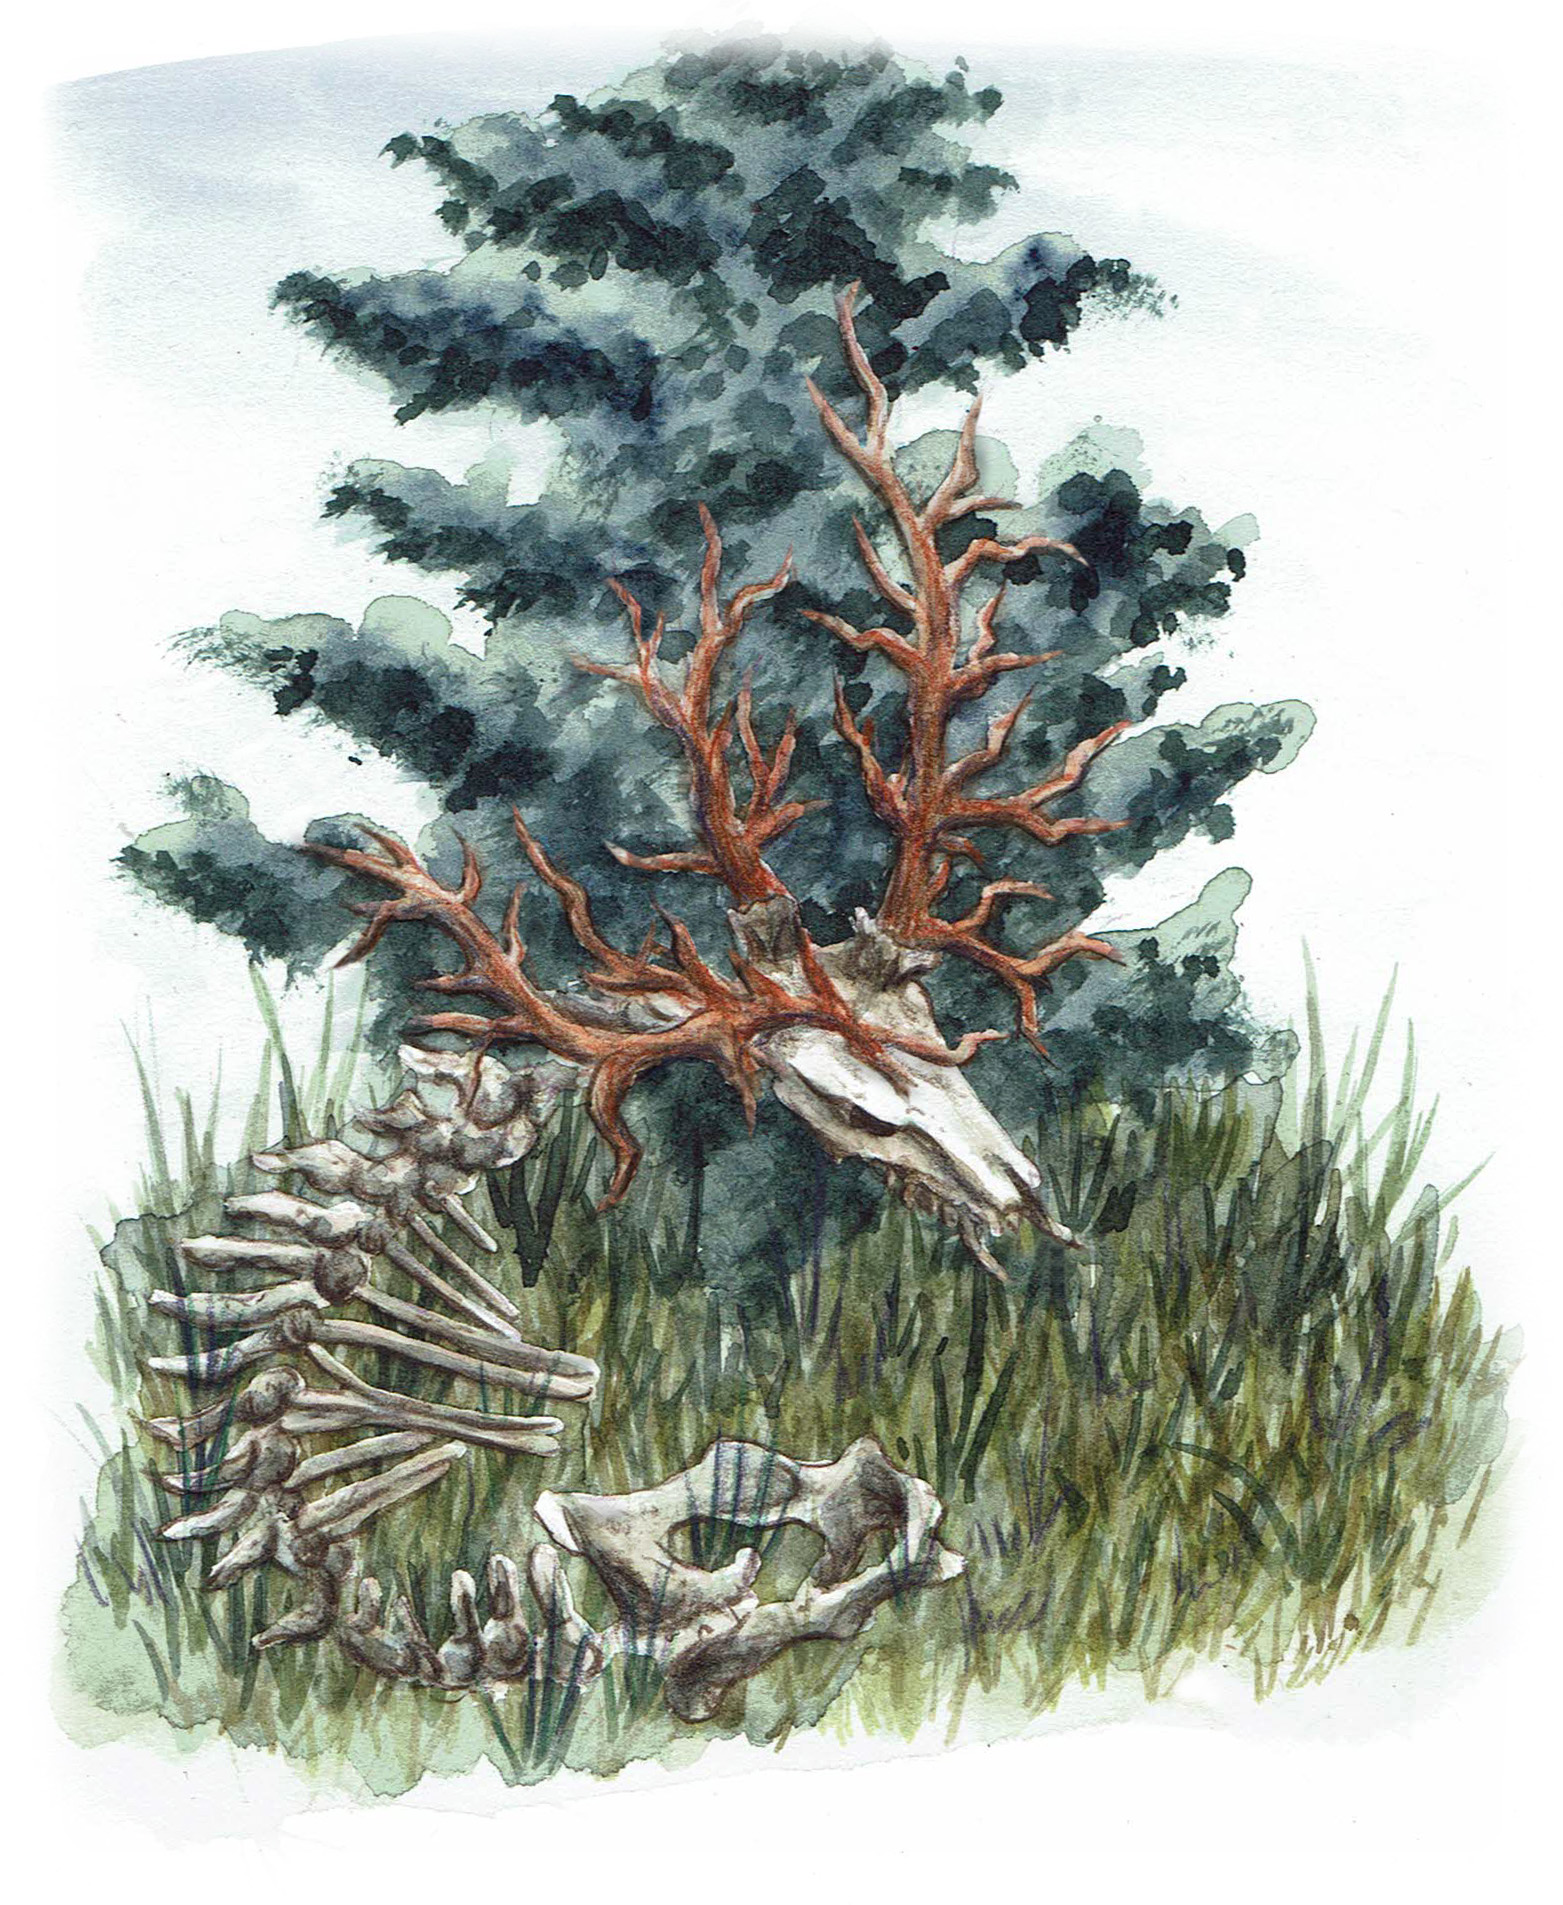
\includegraphics[width=\columnwidth, keepaspectratio]{img/cervide.jpg}

\subsection*{Béhémoth alpin}

Le Béhémoth alpin est le prédateur apex de cette région d'Unterwald. C'est une créature de six mètres de haut (lorsqu'elle se dresse sur ses pattes arrière), avec des caractéristiques ursidées et une lueur malsaine dans le regard.

\textbf{Caractéristiques} : Corps : 11 | Esprit : 4 | Âme : 8

\textbf{Défense passive} : Physique : 16 | Mentale : 9 | Sociale : 13

\textbf{Armes} : Crocs (3), Griffes (2)

\textbf{Protection} : Plaques osseuses (3)

\textbf{Aptitudes spéciales} : 

\begin{itemize}
	\item \textit{Attaque multiple:} Le béhémoth peut attaquer trois fois par round. Deux attaques de griffes et une de crocs.
	\item \textit{Éventrer:} Si le béhémoth réussit ses deux attaques de griffes sur une même cible, il inflige automatiquement 5 points de dommages de corps à la cible, qui ne sont pas diminués par la protection. Si la cible est tuée par cette attaque (ce qui a de fortes chances d'arriver), la cible est littéralement déchirée en deux, et la scène inflige deux points de dommages d'Esprit à toute personne voyant la scène (à moins de réussir un jet d'\textbf{Esprit} à difficulté \textbf{13})
	\item \textit{Peur (4):} La simple vision d'un béhémoth inflige la Peur. Il faut réussir un test d'\textbf{Esprit} à difficulté \textbf{15} sous peine d'être tétanisé par la peur et de perdre \textbf{4} points de la réserve d'esprit. Une réussite à un jet d'\textbf{Esprit} à difficulté \textbf{12} est nécessaire pour sortir de cet état. 
\end{itemize}

\subsection*{Brigand de grand-chemin}

Les routes d'Unterwald sont infestées de brigands de grand-chemin, et les quelques patrouilleurs ne peuvent pas lutter contre la prolifération de ces engeances. Les brigands ne reculeront devant rien pour obtenir les ressources des voyageurs imprudents. On les trouve par groupe de 3 à 6 accompagnés par un chef brigand.

\textbf{Valeur de créature} : 5

\textbf{Défense passive} : 10

\textbf{Armes} : Epée ou hache (2)

\textbf{Protection} : Aucune

\subsubsection*{Chef brigand}

\textbf{Valeur de créature} : 7

\textbf{Défense passive} : 12

\textbf{Armes} : Epée ou hache (2)

\textbf{Protection} : Armure de cuir (1)

\subsection*{Chiroptère}

Les chiroptères sont des monstruosités ailées, de quatre mètres d'envergure, aux griffes acérées et aux crocs suintant un ichor noirâtre empoisonné. Ils attaquent en groupe et tentent d'emporter leurs proies dans les airs en les agrippant avec leurs serres (Automatique dans le cas d'un succès critique). Si c'est le cas, ils montent ensuite à une altitude suffisante avant de laisser la victime retomber dans les rochers (Ce qui tue automatiquement la cible, sauf si elle grille un point de destin)

Dans les autres cas, les chiroptères attaquent avec leurs griffes, leurs serres et leurs crocs (2 attaques par round, au choix du MJ)

\textbf{Valeur de créature} : 8

\textbf{Défense passive} : 13

\textbf{Armes} : Griffes (1), Serres (2) ou Crocs (1 + Poison)

\textbf{Protection} : Aucune

\textbf{Aptitudes spéciales} : 

\begin{itemize}
	\item \textit{Poison:} Sur une attaque de crocs qui inflige des dégâts, la cible doit réussir un test de \textbf{Corps} à difficulté \textbf{12} sous peine d'être empoisonné. Il encaisse un point de dommages de \textbf{Corps} chaque round à son tour jusqu'à réussir le test.
	\item \textit{Peur (2):} Le hurlement des chiroptères inflige la Peur. Il faut réussir un test d'\textbf{Esprit} à difficulté \textbf{13} sous peine d'être tétanisé par la peur. Une réussite à un jet d'\textbf{Esprit} à difficulté \textbf{12} est nécessaire pour sortir de cet état. 
\end{itemize}

\subsection*{Loup sinistre}

Le loup sinistre mesure 1.50 mètre au garrot, et a le dos couvert de longues pointes osseuses rabattues vers l'arrière. Ses yeux sont d'un rouge malsain et ses crocs suintent d'un ichor noirâtre dont le contact inflige des démangeaisons.

Il chasse en meute, de manière organisée, et ciblera toujours l'élément le plus faible d'un groupe, ou le plus dangereux.

\textbf{Valeur de créature} : 7

\textbf{Défense passive} : 12

\textbf{Armes} : Crocs et griffes (1)

\textbf{Protection} : Pointes osseuses (1)

\subsection*{Malandrin}

Le malandrin standard, mal nourri, rebut de caniveau. Il ne trouve du courage qu'en bandes, et ne s'attaquera à un groupe de PJs que si il a l'avantage du nombre.

\textbf{Valeur de créature} : 4

\textbf{Défense passive} : 9

\textbf{Armes} : Poings (1) ou Gourdin (2)

\textbf{Protection} : Aucune

\subsection*{Maraudeur des rochers}

Le Maraudeur des rochers est une créature insectoïde de 2 mètres de haut, aux longues pinces acérées, qui se camoufle dans les rochers d'altitude. Il vit en symbiose avec les béhémoths alpins, rabattant les proies vers l'immense créature.

\textbf{Valeur de créature} : 7

\textbf{Défense passive} : 12

\textbf{Armes} : Pinces (2)

\textbf{Protection} : Chitine (1)

\subsection*{Possédé}

Il n'est pas rare que des voyageurs ayant quitté la route trop longtemps perdent la raison, et s'attaquent aux gens de passage, pris par leur folie furieuse. On nomme ces pauvres âmes des possédés, et il est considéré comme miséricordieux de mettre un terme à leur pénible existence... Même si tuer des humains est toujours difficile.

\textbf{Valeur de créature} : 5

\textbf{Défense passive} : 10

\textbf{Armes} : Poings (1)

\textbf{Protection} : Aucune

\subsection*{Sanglier corrompu}

Le sanglier corrompu a tout du sanglier commun, si ce n'est une taille deux fois supérieure, des poils dorsaux si rèches qu'ils en deviennent acérés, une peau très épaisse et des défenses de 25 centimètres de long d'un vilain jaune. 

S'il est attaqué, son premier réflexe est la charge (qui lui offre un bonus de +2 à l'attaque).

\textbf{Valeur de créature} : 6

\textbf{Défense passive} : 11

\textbf{Armes} : Défenses (2), ignore un point d'armure

\textbf{Protection} : Peau épaisse (1)

\chapter{Scénario : Le Vol de l'Oiseau de Fer}

Situé au bord du Lac de l'Unité, le petit village de l'Envol est protégé des attaques depuis la Chute par l'Oiseau de Fer, une statue de grande taille située au centre du village. Les PJs sont tous des habitants de l'Envol, parfaitement intégrés à leur communauté, et connaissent les légendes liées à l'Oiseau de Fer.

Depuis plusieurs mois, les pillards du Rigg, venus de la rive nord du Lac de l'Unité, ont intensifié leurs raids sur la rive sud, et ont récemment attaqué la ville de Lucarn, à 60 kilomètres à l'ouest. Les rescapés de l'attaque ont rapporté que les pillards se sont montrés d'une sauvagerie sans merci, pillant, violant et réduisant en esclavage tous ceux qui passaient à leur portée.

\section{Vacarme par une nuit d'automne}

Par une nuit sans lune de novembre, tout le village est réveillé par un vacarme métallique au centre du village. Quelques secondes plus tard, le bruit s'intensifie et se déplace vers l'ouest avant de quitter le village.

Lorsque les PJs arrivent sur la place centrale, le constat est accablant. L'Oiseau de Fer n'est plus là.

Les anciens du village se réunissent alors dans la maison commune, et le champ libre est laissé aux PJs pour enquêter de leur côté s'ils le désirent.

Plusieurs indices sont trouvables dans le village.

\begin{itemize}
\item On trouve des traces de pas autour de l'emplacement de l'Oiseau de Fer. Ces traces sont littéralement apparues de nulle part dans la terre meuble. Une des traces est allée directement vers l'Oiseau de Fer.
\item Deux autres traces sont allées vers la porte ouest du village. Les gardes de la porte ouest sont inconscients, les portes sont grandes ouvertes et les murs autour ont été abattus sur quinze mètres de large.
\item Les gardes de la porte sud du village ont entendu un bourdonnement venu du ciel dix minutes avant le fracas au centre du village. Ce bourdonnement semblait venir du sud et a viré vers l'ouest au dessus du village.
\item Trois longues traces droites partent de l'emplacement de l'Oiseau de Fer pour suivre la route de l'ouest, et disparaissent au bout de 800 mètres environ.
\end{itemize}

\textit{Tous les indices semblent montrer que l'Oiseau de Fer s'est envolé vers l'ouest.}

\begin{commentbox}{La vérité sur l'Oiseau de Fer}
L'Oiseau de Fer est un avion de type PC-21. Une relique d'avant la chute, construite non loin de là par \textit{Pegasus}. Une famille de l'Envol, les Klausner, était au fait de ce secret depuis la Chute, et a entretenu l'avion pour le maintenir en état de voler, en accord avec la faction des \textit{Techniciens}.

Il y a 4 mois, Jacques Klausner, un des forgerons du village, est mort d'une maladie débilitante sans avoir pu engendrer d'héritier, ni transmettre son savoir. Les \textit{Techniciens} ont donc parachuté trois agents pour reprendre l'Oiseau de Fer et le conserver.
\end{commentbox}

Suite à leur réunion, les Anciens du village décident de désigner des volontaires (les PJs, comme par hasard) afin d'aller à la recherche de l'Oiseau de Fer. 

\textit{Si certains des PJs rechignent à la tâche, rappelez-leur que l'Oiseau de Fer protège le village, et que tous ceux qu'ils aiment comptent sur eux.}

Il leur est conseillé de partir au petit matin, après avoir pris du repos et des rations.

\onecolumn

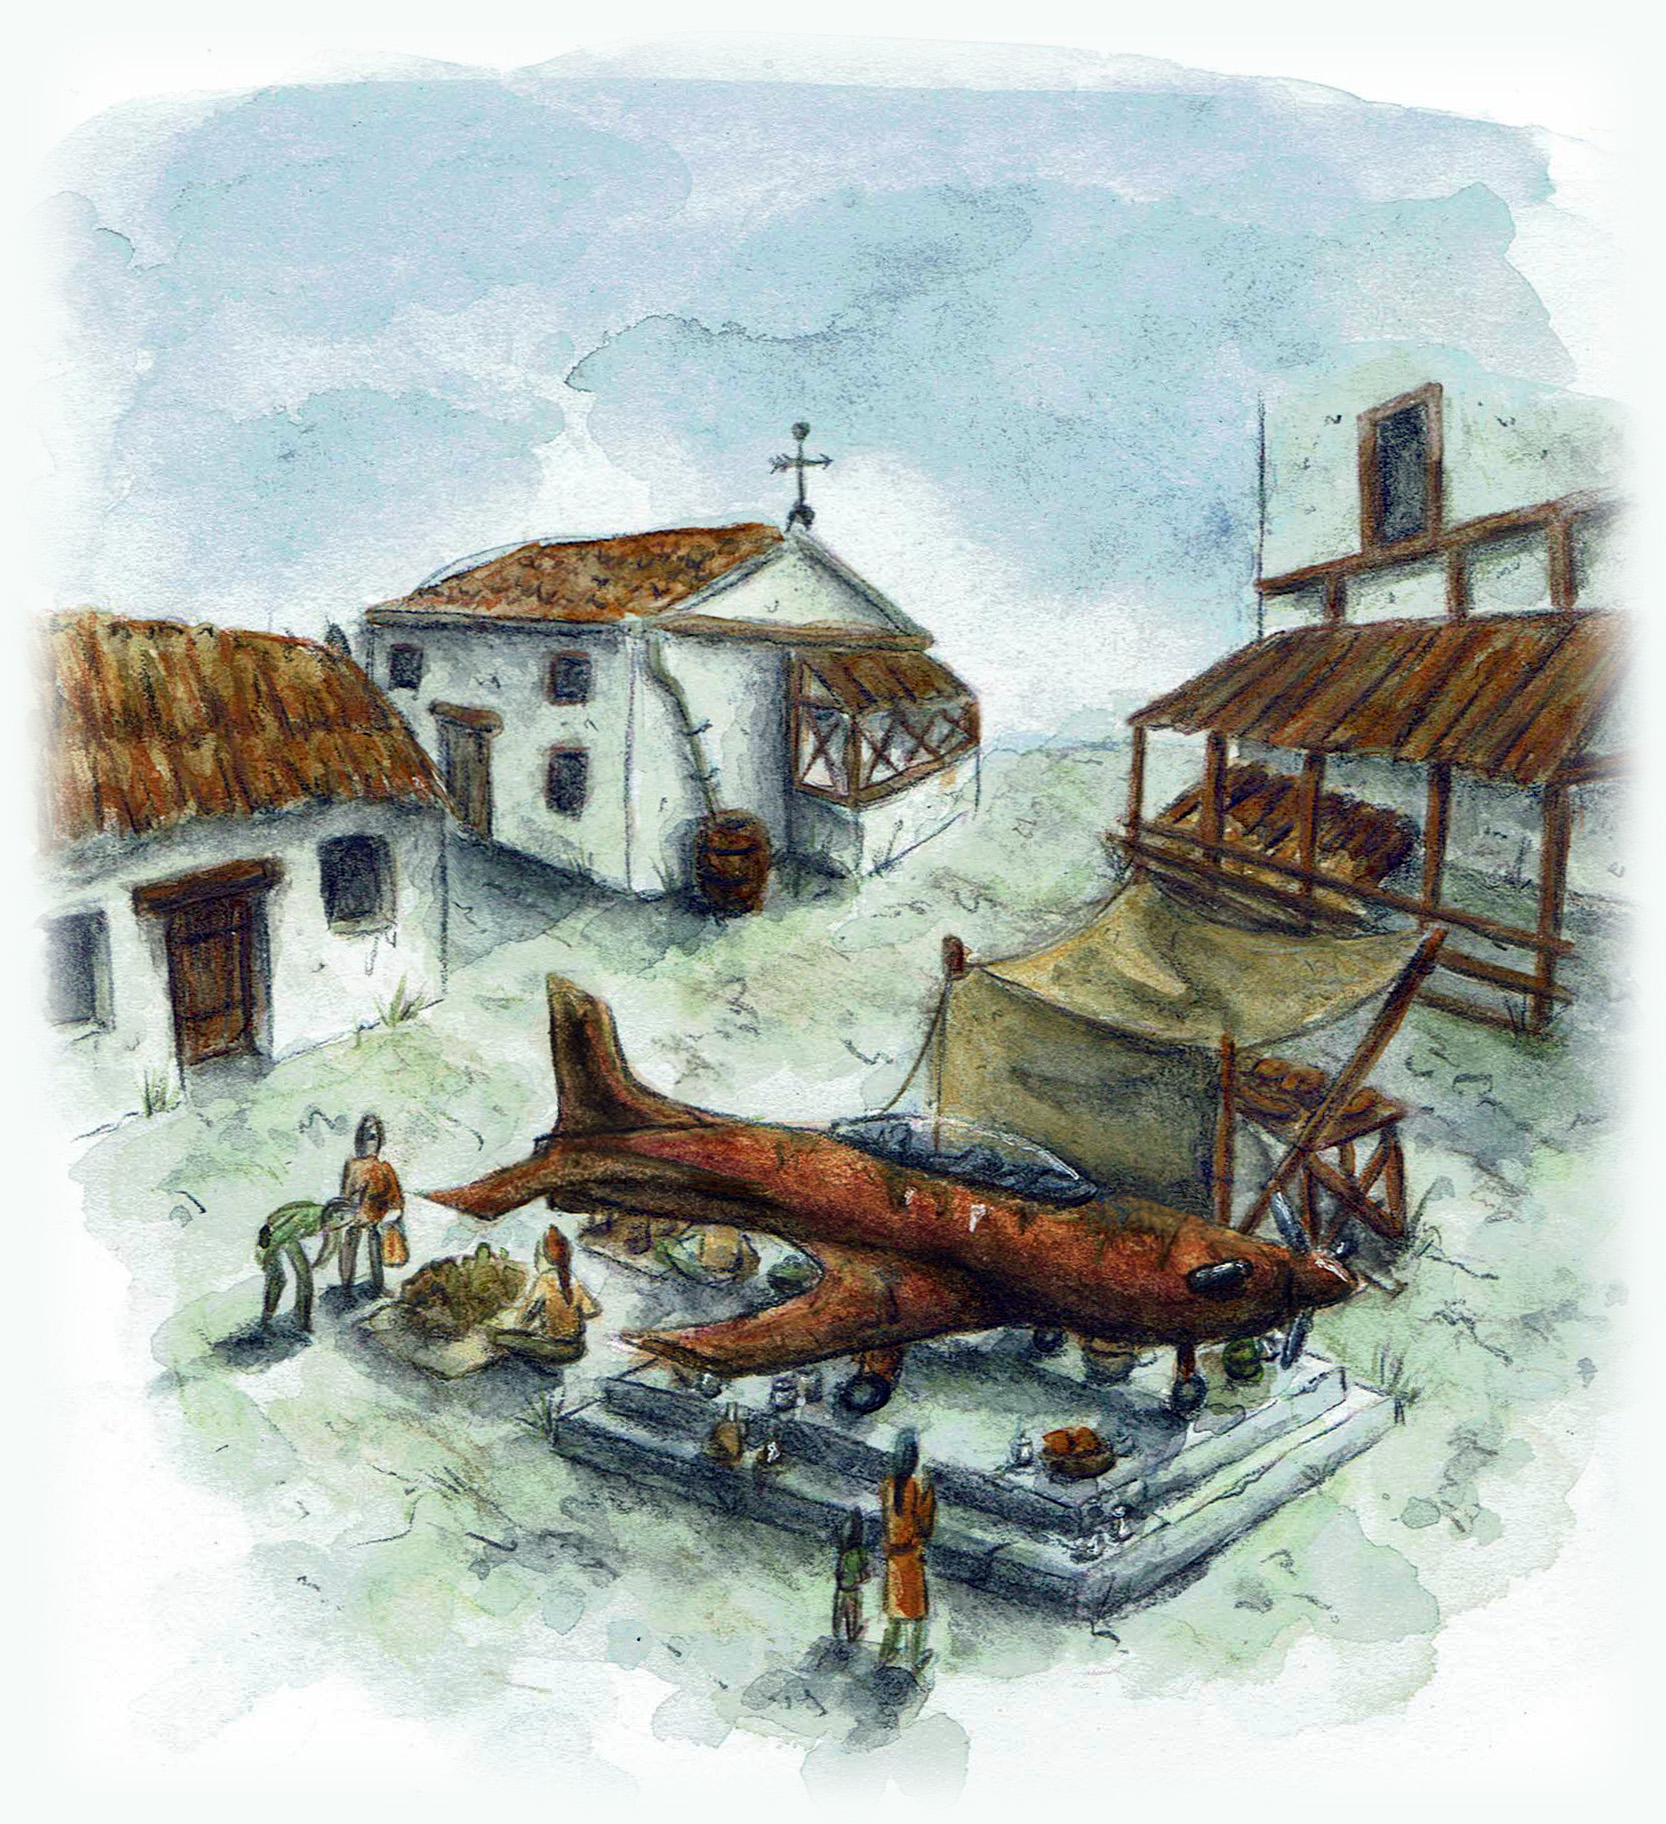
\includegraphics[width=\textwidth, keepaspectratio]{img/village.jpg}

\twocolumn

\section{Sur la route du Nouveau Bastion}

Il faut entre une grosse journée et un jour et demi de marche pour se rendre à la ville la plus proche, le Nouveau Bastion. Il s'agit du principal lieu de commerce de la Basse-Forêt, et la route est \textit{relativement} sûre. Libre à vous d'inclure une ou plusieurs rencontres sur le chemin.

Si les PJs veulent faire la route en une journée, ils doivent réussir un jet de \textbf{Corps + (Athlète/Voyageur)} avec une difficulté de \textbf{14}. Dans le cas où tous les PJs réussissent, alors ils arriveront au Nouveau Bastion alors que la nuit tombe. Dans le cas contraire, ils devront passer une nuit à l'extérieur. Sur un jet d'\textbf{Esprit + (Citadin/Voyageur)} à difficulté \textbf{9}, un PJ peut se souvenir que les ruines du Vieux Bastion se trouvent juste à bonne distance pour passer la nuit dans un lieu sec plutôt que sous la pluie. La rencontre \textit{Nuit au Vieux Bastion} se déclenche alors.

\subsection*{Du mouvement dans le sous-bois}

Alors que les PJs sont sur la route, ils entendent (sur un jet d'\textbf{Esprit + (Eclaireur/Forestier)} à difficulté \textbf{12}) des grognements dans le sous-bois sur leur gauche. Non loin d'eux, un sanglier corrompu est en train de ronger les os d'un cadavre. (Jet d'\textbf{Esprit} difficulté \textbf{10} pour ne pas prendre un point de dommages d'\textbf{Esprit})

Les PJs peuvent choisir de s'écarter, auquel cas la rencontre prend fin, ou d'attaquer le sanglier. En cas de victoire, ils pourront trouver une bourse avec quelques pièces d'argent sur le cadavre.

\subsection*{Un voyageur éreinté}

Vers le milieu de l'après-midi, les PJs rencontrent un homme d'âge mûr qui semble à bout de forces, et qui boîte de la jambe droite. Il les interpelle et leur demande de la nourriture et de l'eau.

Si les PJs se montrent compatissants et aident le voyageur (Il a une vilaine ecchymose à la jambe qui peut être soignée avec un jet de \textbf{Esprit + Médecin} à difficulté \textbf{12}), il se présente à eux sous le nom de \textbf{Rodolf Steinhof}. Il s'agit d'un ancien forgeron de la ville de Lucarn, qui a évité l'attaque de la ville par les pillards du Rigg alors qu'il était en visite chez son fils \textbf{Jakob} au Nouveau Bastion. Il a appris que L'Envol a récemment perdu son forgeron, et a décidé de prendre la route pour se présenter au village.

Si les PJs l'ont aidé, il leur remet une lettre d'introduction auprès de son fils, ce qui leur permettra de ne pas avoir à séjourner dans une des auberges de la ville. Par ailleurs, il se montrera très reconnaissant si les PJs font de même pour le conseil du village, et leur remettra une hachette ou une dague de sa fabrication (Bonne qualité, +1 pour toucher)

\subsection*{Une lueur dans la pénombre}

Peu avant le crépuscule (soit avant d'arriver au Vieux Bastion, soit, si les PJs ont réussi à faire la route en une journée, avant d'arriver au Nouveau Bastion), le regard d'un PJ (déterminé au hasard ou au bon vouloir du MJ) est attiré par une lueur provenant des bois. Il doit réussir un jet d'\textbf{Esprit} à difficulté \textbf{12} pour ne pas prendre la direction de cette lueur. 

Si les autres PJs tentent de l'empêcher de s'y rendre, ils doivent également réussir le jet d'\textbf{Esprit}.

La lueur provient d'un petit étang qui émet une légère luminescence. Les PJs ayant approché peuvent y boire une eau fraîche et au léger goût herbacé. Tout PJ ayant bu l'eau de l'étang doit réussir un jet de \textbf{Corps} à difficulté \textbf{15} ou tomber dans une transe hypnotique. ()\textit{Voir encadré ci-dessous})

\begin{commentbox}{La transe de l'étang lunineux}
	Tout personnage ayant succombé à la transe se retrouvera dans un paysage méconnaissable, où chariots de fer fortement bruyants et hautes demeures d'une pierre lisse se côtoient. 
	
	\textit{(Note pour le MJ: Ils voient le monde d'avant la Chute, n'hésitez pas à décrire un paysage urbanisé de montagne européenne aux alentours des années 2010, à les perdre dans des rues et ruelles où la forêt n'a pas repris sa place.)}

	Lorsqu'ils se réveillent de leur transe, ils sont en plein milieu des bois, sans points de repère. Il faudra plusieurs jets d'\textbf{Esprit + Eclaireur/Voyageur} pour retrouver la route. Le MJ peut ajouter une ou plusieurs rencontres hostiles sur le chemin s'il le désire. Il se peut que les PJs aient à passer la nuit dehors.
\end{commentbox}

\subsection*{Nuit au Vieux Bastion}

Si les PJs ont choisi de passer la nuit au Vieux Bastion, ils arrivent peu de temps avant que la nuit ne soit complètement tombée. Alors qu'ils entrent dans la ville en ruines, faites jeter un jet de \textbf{Corps + Athlète} de difficulté \textbf{10} au PJ qui ouvre la marche. S'il échoue, il trébuche sur une longue pièce de métal \textit{(un rail de chemin de fer)} cachée dans les herbes hautes.

Après quelques minutes de recherche, ils trouvent un bâtiment approprié pour passer la nuit. Ce bâtiment date d'avant la chute, et est caractérisé par ses murs de pierre lisse et unie. Le rez-de-chaussée peut être facilement barricadé à l'aide de planches et de tôles que les PJs trouveront à l'intérieur. L'étage supérieur, quant à lui, ne possède que trois murs, et a une hauteur sous plafond de 10 mètres. \textit{(Il s'agit d'une ancienne station basse de téléphérique)} Il sera donc difficile de le barricader entièrement. Les PJs ont donc tout intérêt à s'abriter au rez-de-chaussée.

\textbf{INSERT MAP HERE}

Durant la nuit, ils sont attaqués par plusieurs loups sinistres \textit{(Entre 2 et 4, selon le nombre de PJs et la difficulté désirée)} qui passent par le trou béant à l'étage. Laissez aux PJ plusieurs actions de préparation alors que les loups s'attaquent à la porte en haut de l'escalier.

\section{Le Nouveau Bastion}

Les PJ arrivent au Nouveau Bastion à la toute fin de journée s'ils ont réussi à faire le trajet depuis l'Envol en un jour, ou vers midi le lendemain. Trouver des informations sur ce qui s'est passé la nuit précédente (ou celle d'avant) n'est pas extrêmement complexe, néanmoins il faut convaincre les citadins d'adresser la parole à des bouseux, surtout en ces temps troublés où les raids des pillards sont nombreux.

Libre aux PJs de choisir leur manière d'aborder les habitants du Nouveau Bastion, que ce soit en payant des verres dans une taverne, en glissant la pièce à des mendiants, ou en allant trouver la garde. Un roleplay approprié et/ou un jet d'\textbf{Âme + Citadin/Orateur} peuvent faciliter ou rendre plus ardu l'obtention des informations.

Les informations que les PJs peuvent obtenir sur place sont les suivantes :

\begin{itemize}
	\item La nuit de la disparition de l'Oiseau de Fer, un grondement métallique a été entendu au dessus du Nouveau Bastion. Le bruit venait de l'est, et a obliqué vers le sud, en direction du Col Brun.
	\item Des rescapés de la ville de Lucarn racontent le pillage de la ville. \textit{(Voir l'événement "Lucarn a brûlé")}
	\item Une caravane de marchands part pour la région de la Haute-Forêt le lendemain vers le milieu de journée. Les PJs peuvent s'y joindre, à condition d'aider à la défendre en cas de besoin.
\end{itemize}

\subsection*{Une nuit en ville}

Les PJs peuvent décider de repartir au plus vite, mais c'est particulièrement déconseillé. Ils sont sans doute fatigués ou blessés. Il est donc plus sage pour eux de rester au moins une nuit au Nouveau Bastion.

Si ils sont venus en aide à \textbf{Rodolf Steinhof} lors de leur voyage depuis l'Envol, ils peuvent aller trouver \textbf{Jakob Steinhof}, un des forgerons de la place du marché. Celui-ci les accueillera avec plaisir et leur offrira gite et couvert, et leur proposera également de faire affaire à \textit{prix d'ami}.

Dans le cas contraire, ils doivent passer la nuit dans une auberge mal famée, \textbf{Le Chaudron bosselé}, toutes les auberges correctes étant occupées par des réfugiés de Lucarn. Il est possible qu'une bagarre ou une agression ait lieu dans l'auberge. Utilisez le profil des malandrins du bestiaire.

\subsection*{Lucarn a brûlé}

Alors qu'ils se promènent sur la place du marché du Nouveau Bastion, les PJs sont interpelés par un homme d'une trentaine d'années, au regard hanté. Il est un des survivants du pillage de Lucarn, ou comme il le dit, le massacre de Lucarn.

Si les PJs lui accordent de l'attention, il leur raconte les moindres détails de l'attaque sur la ville autrefois prospère de l'ouest du Lac de l'Unité.

\begin{commentbox}{Le massacre de Lucarn}
	La ville de Lucarn a été attaquée par les pillards du Rigg il y a deux semaines et demi. Quelques jours auparavant, des pillards étaient arrivés en ville sous couvert d'une caravane marchande. 

	La nuit de l'attaque, les pillards infiltrés ont tué les gardes qui surveillaient la porte nord pour laisser entrer les leurs, pendant qu'une autre vague attaquait par le lac. Plus de cinq cents brigands ont alors attaqué la ville, et s'en sont rendus maîtres en moins de trois heures malgré la résistance farouche de la garde, en nette infériorité numérique.

	Le pillage en tant que tel a duré deux jours, pendant lesquels les pillards ont torturé les citadins pour connaître l'emplacement de leurs richesses, ne reculant devant aucune atrocité pour arriver à leurs fins.

	La moitié des habitants a été réduite en esclavage et emmenée par bateau, tandis qu'une grande partie de la population restante a été massacrée sur place. Seuls ceux qui ont réussi à se cacher des pillards a pu survivre, avant que leur ville ne soit incendiée. La ville n'est plus que ruines fumantes à présent.
\end{commentbox}

\textit{Note pour le MJ: Vous pouvez décrire avec autant de détails ce que le rescapé a vu. Cela dit, n'oubliez pas que ce genre de scène est désagréable et choquante. Ayaez pitié de vos joueurs}

Le rescapé du massacre a pu sa cacher dans une cave à moitié murée lors du massacre, mais sa femme et ses deux filles ont été emmenées en tant qu'esclaves par les pillards. C'est un homme brisé qui a tout perdu.

\subsection*{Une caravane pour le Col Brun}

La route du Col Brun est réputée pour être très dangereuse, et il est rare qu'un groupe de voyageurs s'y aventure sans bonne garde ou sans une bonne raison. Une fois par mois environ, des marchands se réunissent en une caravane de plusieurs chariots et engagent des gardes aguerris.

Il n'est pas rare que les voyageurs rejoignent ces caravanes pour assurer leur sécurité. Il s'agit normalement d'une prestation payante (et assez chère), néanmoins il est possible de négocier avec un test d'\textbf{Âme + Marchand/Orateur} pour se faire engager comme gardes supplémentaires, ce qui peut rapporter un petit pécule.

Le chef de caravane est un certain \textbf{Michel Klov}, un homme bedonnant d'une quarantaine d'année à l'oeil vif et au nez aquilin.

\section{La route du Col Brun}

Si les PJs ont choisi de rejoindre la caravane, la route sera particulièrement tranquille, la présence des gardes armés en nombre éloignant naturellement les bandits et la plupart des bêtes sauvages. Un MJ taquin pourra cependant créer une ou deux rencontres avec des bandits ayant perdu la raison (Cela ne devrait toutefois pas mettre en danger la peau des PJs)

Dans le cas où ils ont pris la route du Col sans escorte, alors le MJ sera bien inspiré de leur faire comprendre leur erreur.

\subsection*{Au sein de la caravane}

La route du Col Brun passe par plusieurs localités. Tout d'abord le village d'Alp, engoncé dans la vallée entre le Pic du Pilat et la Corne de Bastion. Il s'agit d'un village de taille équivalente à l'Envol, mais la principale richesse de celui-ci n'est pas l'agriculture, mais l'exploitation de la pierre des carrières proches.

La journée suivante mène la caravane jusqu'au bourg fortifié de Serment, au bord du lac du même nom. L'auberge est petite, mais peut tout de même accueillir l'intégralité de la caravane, et la soirée est passée à discuter des derniers événements avec les locaux.

Le passage des deux communautés de Gisville et de Longères se fait également dans le calme, et ils arrivent au pied des montagnes.

La caravane repart le lendemain pour le passage du Col, qui aura lieu dans la fin d'après-midi ou le début de la soirée.

\textit{Note pour le MJ: Cette portion de route devrait permettre aux PJs de se reposer, et de panser leurs blessures avant le passage du Col qui constitue le plus grand danger de ce scénario.}

\subsection*{En route sans escorte}

Si les PJs ont choisi de voyager sans escorte, ils vont se heurter à la défiance, voire l'hostilité des villageois d'Alp, et à une certaine méfiance de la part des habitants de Serment. En effet, même s'ils n'ont pas quitté leur province (la Basse-Forêt), ils sont loin de leur village, et sont de parfaits inconnus pour les locaux.

Ils peuvent toutefois apprendre (s'ils ne se font pas chasser avec des fourches et des torches) que les habitants des deux communautés ont entendu un grondement métallique se dirigeant vers le sud plusieurs nuits auparavant. Les gardes de Serment l'ont consigné dans leur rapport quotidien. Ils sont sur la bonne voie.

Les habitants de Gisville et de Longères sont tout aussi rechignants à donner des informations.

Ils peuvent également apprendre que le Col est infesté de créatures plus dangereuses et aggressives les unes que les autres. Il est plus sûr de passer le Col de nuit, paradoxalement, car seuls les chiroptères sont susceptibles d'attaquer de nuit, contrairement aux créatures diurnes.

\textit{Note pour le MJ: Vos joueurs ont choisi de faire la route tous seuls ? Tant pis pour eux, pas de repos pour les braves.}


\section{Le passage du Col Brun}

\subsection*{Au sein de la caravane}

Il est près de 16 heures lorsque la caravane arrive au pied de la route du col. Michel Klov fait arrêter le groupe, et donne ses instructions pour le passage du col, qui est la partie la plus dangereuse de la route.

La région du Col Brun est infestée de chiroptères, des monstres ailés de quatre mètres d'envergure. Tous les membres de la caravane doivent monter dans les chariots et les archers doivent se préparer à faire feu sur toute créature tentant d'approcher. En aucun cas la caravane ne doit s'arrêter. Si une personne tombe d'un chariot, elle doit se débrouiller seule pour remonter à bord. Il n'y aura aucune tentative de sauvetage, et, il insiste, cela vaut également pour lui-même.

Si on lui demande pourquoi le passage du col se fait de nuit et non de jour, Klov répondra que la nuit permet de ne risquer "que" d'affronter les Chiroptères. Des créatures plus massives et aggressives rôdent autour de la route en journée.

La caravane entame sa longue et difficile ascension vers le Col Brun, dont le dénivellé est d'environ 400 mètres. La route est difficile avec les chariots chargés, mais les boeufs et chevaux de trait progressent malgré tout.

Après deux heures, alors que les chariots dépassent la limite des arbres et arrivent dans une zone plus rocailleuse, les PJs réussissant un jet d'\textbf{Esprit + Eclaireur/Voyageur} à difficulté \textbf{12} remarquent que plusieurs des pierres le long du chemin sont en fait des ossements, tant humains que d'animaux. Cette vision macabre leur inflige un point de dommages d'\textbf{Esprit} à moins de réussir un jet à difficulté \textbf{12}.

La nuit tombe alors que la route se fait plus pentue et serpente sur les flancs escarpés de la montagne. Des torches sont allumées sur tous les chariots, et l'ambiance se fait de plus en plus pesante. Alors que la caravane approche du col, des crissements stridents retentissent dans les ténèbres, glaçant le sang de l'équipée. (Jet d'\textbf{Esprit} à difficulté \textbf{13} pour ne pas subir \textbf{2 dommages d'Esprit} et être tétanisé de peur jusqu'à réussir un jet d'\textbf{Esprit} à difficulté \textbf{12}).

Un vol de Chiroptères est en train de fondre sur la caravane. (\textit{Note pour le MJ: Il s'agit du combat qui forme le climax du scénario, alors n'hésitez pas à le rendre aussi difficile que vous le désirez. Les chiroptères sont des adversaires coriaces, aussi vous pouvez en compter en moyenne un pour 3 combattants (ou PJ), en incluant les gardes de la caravane.})

Lorsque le combat s'achève, ils passent la stèle qui marque le passage du Col Brun, et s'engagent dans la descente vers les terres de la Haute-Forêt. 

\subsubsection*{Sans escorte}

Sans escorte, les PJs peuvent passer le col de jour ou de nuit, à choix. S'ils ont réussi à discuter avec les villageois sur le chemin, ils ont appris que le Col est plus dangereux de jour que de nuit. 

Traitez la montée vers le col comme avec la caravane, et préparez la rencontre suivante :

\begin{itemize}
	\item Si les PJs passent le col de nuit, entre 3 et 5 chiroptères
	\item Si ils passent le col de jour, préparez-vous à un TPK, et envoyez-leur deux maraudeurs des rochers et un béhémoth alpin. (Ils ont ignoré les avertissements et ont choisi la manière dure. Ils seraient bien inspirés de fuir cela dit.)
\end{itemize}

Dans le cas où ils survivent, ils passent le col au moment où le combat s'achève, et vous pouvez passer à l'épilogue.

\section{Un oiseau en cage}

Les premières lueurs de l'aube (ou la fin de l'après-midi si le passage du col s'est fait en journée) dévoilent la douce beauté de la vallée de la Haute-Forêt, et la lumière du soleil se reflète sur le lac de Brillance en contrebas. 

Les PJs entendent alors un grondement métallique, et voient surgir d'une vallée encaissée non pas un, mais trois oiseaux de fer, tous identiques, qui s'envolent rapidement vers les nuages et y disparaissent. Cette vallée est encore à deux bons jours de marche, mais il serait stupide de ne pas prendre de repos dans la ville de Brillance. Après tout, ils ont survécu à l'une des routes les plus dangereuses de la région.

\subsection*{Repos à Brillance}

Ils arrivent en ville à la fin de la journée. Brillance est une bourgade un peu plus grande que le Nouveau Bastion, située au bord d'un lac poissonneux. Si les PJs ont accompagné la caravane, ils sont remerciés par le chef de celle-ci pour leur aide, et se voient remettre une bourse avec quelques pièces d'argent.

En ville, ils peuvent obtenir les informations suivantes :

\begin{itemize}
	\item La vallée d'où ils ont vu émerger les oiseaux de fer est habitée par un groupe sectaire, très fermé, qui a investi la vallée de Sémiombre voici plusieurs décennies.
	\item Il est très dangereux de s'introduire dans cette vallée sans y être invité. Pour être exact, aucune personne n'est revenue après y être entrée.
	\item Il est possible de discuter avec un membre de la secte qui a été capturé par la garde, il est détenu à Villars-de-Brillance.
\end{itemize}

\subsection*{Discussion avec un Technicien}

L'homme emprisonné à Villars-de-Brillance est habillé d'une curieuse combinaison bleue, avec un symbole représentant une roue dentée. Il est d'assez mauvaise composition lorsqu'on essaie de lui parler. Néanmoins, avec beaucoup de patience et de persuasion, il est possible de lui arracher les informations suivantes :

\begin{itemize}
	\item Il donne le nom de sa faction : Les Techniciens.
	\item Il est très hautain lorsqu'on lui pose des questions sur l'Oiseau de Fer, et répond qu'il est mieux entre les mains des siens, et que des pouilleux ignares ne devraient pas toucher aux reliques.
	\item Si les PJs se résolvent à le torturer, ils peuvent obtenir un itinéraire caché pour rejoindre la vallée. Néanmoins, le chemin est dangereux, et les Techniciens gardent leurs secrets farouchement.
\end{itemize}

\subsection*{Vers la vallée de Sémiombre}

\subsubsection*{Par la route}

Si les PJs se rendent à la vallée de Sémiombre par la route, ils se heurteront à la vigilance des gardes des Techniciens, qui les repousseront fermement loin de leur domaine.

\subsubsection*{Par le chemin caché}

Le chemin dissimulé mène les PJs jusqu'à une caverne de la vallée, où ils peuvent observer un grand nombre de Techniciens en combinaison bleue s'affairer autour de nombreux oiseaux de fer de formes différentes.

\section{Epilogue}

Si les PJs passent à l'attaque, ils se font capturer ou tuer par les gardes. Ils peuvent aussi se révéler, auquel cas ils se feront capturer, et emprisonner, avant d'être relâchés en un lieu complètement inconnu.

Si ils choisissent de rebrousser chemin, le monde périlleux d'Unterwald s'ouvre à eux, et, même s'ils ne ramènent pas l'Oiseau de Fer à leur village, ils savent à présent qu'il s'agit d'une relique de l'ancien temps et non d'une statue protectrice.

Quelle que soit la solution choisie par les PJs, la suite de cette histoire se déroule dans la campagne d'Unterwald, qui leur fera découvrir les secrets du Monde d'avant, et rencontrer d'autres factions plus terribles les unes que les autres.

\section{Personnages prétirés}

Tous les personnages prétirés de ce livre peuvent-être de n'importe quel sexe. En effet, Unterwald est suffisamment sombre et dangereux pour que ses habitants aient perdu le luxe du sexisme.

Pour cette raison, aucun personnage n'a de nom, ni de description. C'est à vous, joueurs, de vous approprier votre personnage et de le personnaliser comme bon vous semble.

Six personnages prétirés sont disponibles ici, chacun avec leur spécialité. 

\begin{itemize}
	\item Un chasseur à l'oeil vif
	\item Un herboriste grincheux
	\item Un marchand généreux
	\item Un soldat aguerri
	\item Un touche-à-tout beau parleur
	\item Un voyageur endurci
\end{itemize}

\subsection*{Chasseur à l'oeil vif}

\textbf{Crainte :} Se retrouver \textit{perdu} sans repère.

\textbf{Réconfort :} Une griffe de loup sinistre en pendentif.

\textbf{Corps : 6 | Esprit : 6 | Âme : 5}

\textbf{Traits :} Chasseur +2 | Athlète +1 | Forestier +1

\textbf{Equipement :} Un arc et des flèches (Dommages 2 ; Portée longue) ; Un couteau de chasse (Dommages 1) ; Des rations de viande séchée ; Un manteau en toile cirée

\subsection*{Herboriste grincheux}

\textbf{Crainte :} Voir un endroit où la nature est morte

\textbf{Réconfort :} Un herbier relié

\textbf{Corps : 5 | Esprit : 7 | Âme : 5}

\textbf{Traits :} Médecin +2 | Forestier +1 | Paysan +1

\textbf{Equipement :} Une serpe (Dommages 1) ; Une sacoche pleine d'herbes médicinales (+1 pour guérir des blessures légères)

\subsection*{Marchand généreux}

\textbf{Crainte :} Se retrouver sans le sou

\textbf{Réconfort :} Une pièce de monnaie datant d'avant la Chute

\textbf{Corps : 5 | Esprit : 6 | Âme : 6}

\textbf{Traits :} Marchand +2 | Citadin +1 | Administrateur +1

\textbf{Equipement :} Une dague (Dommages 1) ; Un grand sac contenant des objets de menue valeur

\subsection*{Soldat aguerri}

\textbf{Crainte :} Être enfermé sans possibilité de fuir

\textbf{Réconfort :} Une mèche de cheveux blonds dans un mouchoir

\textbf{Corps : 7 | Esprit : 5 | Âme : 5}

\textbf{Traits :} Soldat +2 | Athlète +1 | Bagarreur +1

\textbf{Equipement :} Une hallebarde (Dommages 3) ; Une armure de cuir (Protection 1) ; Une paire de dés en os

\subsection*{Touche à tout beau-parleur}

\textbf{Crainte :} Devoir dormir à l'extérieur

\textbf{Réconfort :} Un portrait peint sur une planchette en bois

\textbf{Corps : 5 | Esprit : 5 | Âme : 7}

\textbf{Traits :} Intrigant +2 | Larron +1 | Saltimbanque +1

\textbf{Equipement :} Un stylet (Dommages 1 - Ignore 1 point d'armure) ; Un bracelet en argent ; Une lanterne sourde

\subsection*{Voyageur endurci}

\textbf{Crainte :} Devoir quitter la route

\textbf{Réconfort :} Une carte de la région sur une peau

\textbf{Corps : 6 | Esprit : 5 | Âme : 6}

\textbf{Traits :} Voyageur +2 | Soldat +1 | Ferrailleur +1

\textbf{Equipement :} Une épée (Dommages 2) ; Un nécessaire de dessin ; Une épaisse pèlerine de laine

\chapter{Crédits et remerciements}

\section*{Crédits iconographiques}

Toutes les illustrations ont été créées par la talentueuse Diane Georges. Vous pouvez retrouver ses travaux sur \url{https://diane-georges.net}

\section*{Remerciements}

Je remercie ma compagne, Elodie Armbruster, pour son soutien indéfectible pendant l'écriture de ce kit, et la création de ce jeu de rôle.

J'adresse un merci tout particulier à Diane, qui a réalisé les illustrations de ce kit.

Je remercie également mes chers amis, Raph et Adrien, pour leurs conseils, critiques et remarques.

Enfin je remercie tous les playtesteurs qui m'ont aidé à affiner ce scénario durant l'année 2019, au cours des nombreuses conventions où je l'ai fait jouer.

\end{document}